% !TeX root = ../main.tex
\chapter{Related Work}\label{chapter:related-work}


% ModControl – Mobile Phones as a Versatile Interaction Device for Large Screen Applications
%\section{Mobile Phones as a Versatile Interaction Device for Large Screen Applications}\label{section:mobile-phones-interaction-device-large-screen}
\section{Deller et al.}\label{section:deller-2011}
\citeauthor{Deller.2011} propose a modular framework to enable multi-user interactions between smartphones and large-screen applications. A typical client-server architecture with an XML\footnote{XML is a standardized data exchange format, that uses human-readable text.}-based protocol is used. They differentiate between application clients (the large screen) and interaction clients (the smartphones)~\cite{Deller.2011}.

The client app is provided with different modules. Some modules offer similar functionality to the experiments implemented in this thesis: Their text module enables users to enter a text; Their accelerometer/magnetometer module sends \gls{IMU} data like acceleration and magnetic field data in the background to the server. They also described how they integrated their framework in an application where users can navigate a map and toggle display settings~\cite{Deller.2011}.

The approach presented in this thesis uses a similar architecture. Not only the client-server structure is similar, but also the modularized abstraction is used in so-called \enquote{Interactions}.


% Phone-based motion control in VR (Klinker)
%\section{Phone-based Motion Control in VR}\label{section:phone-based-motion-control-vr}
\section{Benzina et al.}\label{section:benzina-2011}
\citeauthor{Benzina.2011} introduce a system for flying through \glspl{VE} by using a smartphone as input device.
% Since the sight is occluded by the \gls{HMD}, the phone display cannot be used to display information.
They try to find convenient mappings between the users' actions with the mobile phone and the subsequent reactions in the \gls{VE}. To solve this, they investigate the \glspl{DOF} required to implement a quickly learnable and comfortable travel task.

Different methods using the accelerometer, magnetic field sensor, and touch screen for controlling the flight movement are presented and evaluated. They concluded that the most accurate method for controlling the flight uses an approach where an airplane metaphor (four \glspl{DOF}) is simulated~\cite{Benzina.2011}.

\citeauthor{Benzina.2011} use the orientational and the touch screen data, the phone provides, to control a \gls{VE}, as is done in this thesis.


% Mobile Devices for Interaction in Immersive Virtual Environments
%\section{Mobile Devices for Interaction in Immersive Virtual Environments}\label{section:mobile-devices-interaction-ve}
\section{Dias et al.}\label{section:dias-2018}
\citeauthor{Dias.2018} propose a solution where the smartphone has a visual representation in \gls{VR}. The visual representation displays information and a \gls{UI} on its virtual screen. The camera in the smartphone tracks a marker on the \gls{HMD} to track its own position relative to the headset. The setup is shown in Figure~\ref{fig:dias-2018}.

\begin{figure}[H]
	\centering
	\begin{subfigure}[t]{0.48\textwidth}%
		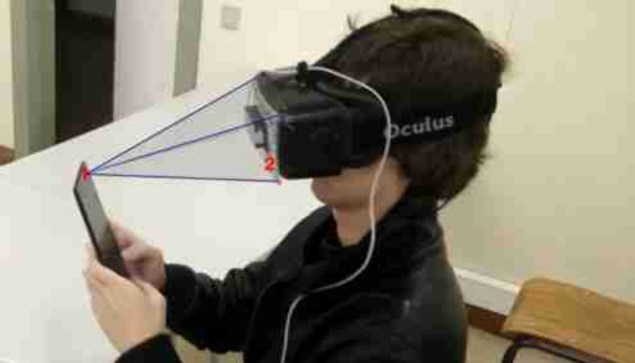
\includegraphics[width=\textwidth]{figures/related_work/dias_2018_tracking.png}
    \caption{The front camera of the smartphone tracks the marker on the \gls{HMD}.
    \newline{}
    Source:~\cite[Figure 3]{Dias.2018}
    }\label{fig:dias-2018-tracking}% chktex 9 % chktex 10
	\end{subfigure}%
	\hspace{0.04\textwidth}%
	\begin{subfigure}[t]{0.48\textwidth}%
		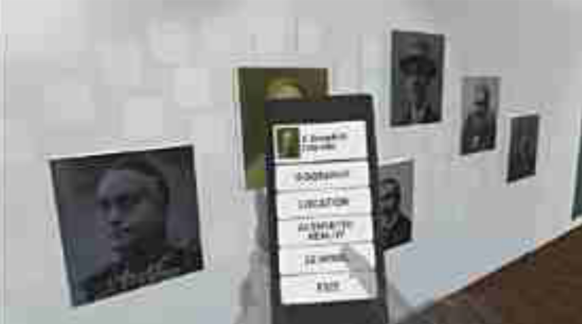
\includegraphics[width=\textwidth]{figures/related_work/dias_2018_virtual_smartphone.png}
    \caption{The virtual smartphone representation and hand avatar in the \gls{VE} while interacting with the \gls{UI}.
    \newline{}
    Source: Adapted from~\cite[Figure 5]{Dias.2018}
    }\label{fig:dias-2018-virtual-smartphone}
	\end{subfigure}%
	\caption[Tracking setup by Dias et al.]{The tracking system by \citeauthor{Dias.2018}~\protect\cite[4,5]{Dias.2018}.}\label{fig:dias-2018}
\end{figure}

Because users interacts with the \gls{UI} using the touch screen of the smartphone as they would do in real life, the fingers have to be tracked and visualized. Otherwise, users would not know where their fingers are going to hit the touch screen because the sight is occluded physically by the \gls{HMD}. To solve this problem, they attach a Leap Motion sensor to the \gls{HMD}, which tracks the fingers and displays a hand avatar~\cite{Dias.2018}.

Almost the same research team (\citeauthor{Afonso.2017}) evaluated a selection task using a tablet as an input device in \gls{VR} using the same \gls{VR} setup. They compare the selection time of users selecting a button on the tablet using a realistic hand avatar, a translucent hand avatar, and without any avatar of the hand. Surprisingly, the evaluation shows that users performed the best without any virtual avatar. The authors explain that this is due to the tracking inaccuracies of the tablet and hand. However, users made fewer selection errors when an avatar was displayed~\cite[247-248]{Afonso.2017}.

Those papers are especially useful for the research of this thesis because they introduce a visual representation of the smartphone in \gls{VR}, which is used in this thesis, too. 


\section{Katzakis et al.}\label{section:katzakis-2010}
An application to view three-dimensional models controlled with a smartphone was implemented by \citeauthor{Katzakis.2010}. Their approach uses a smartphone to rotate a model which is displayed on a conventional display~\cite[139]{Katzakis.2010}. 

The phone is wirelessly connected to a computer where the model is rendered. The orientation data is provided by the \gls{IMU} of the smartphone and, once calibrated to the screen position, is directly mapped to the model, as seen in Figure~\ref{fig:katzakis-2010}~\cite[139]{Katzakis.2010}. 

\begin{figure}[H]%
  \centering%
  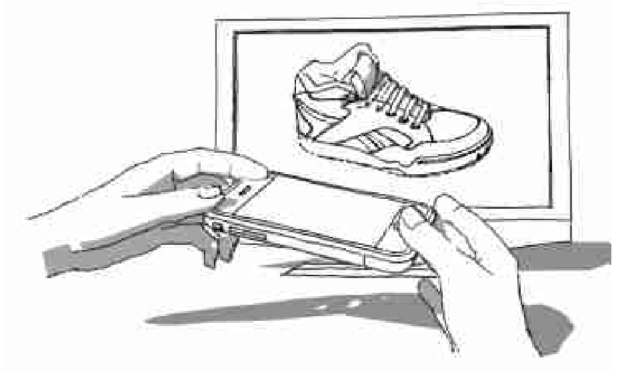
\includegraphics[height=6cm]{figures/related_work/katzakis_2010_3d_object.png}%
  \caption[Model viewer implementation by Katzakis et al.]{
  The model viewer implementation by \citeauthor{Katzakis.2010}. The smartphone is rotated, to orient the three-dimensional model on the display.
  \newline{}
  Source:~\cite[Figure 1]{Katzakis.2010}}\label{fig:katzakis-2010}
\end{figure}

In the evaluation of their system, a mouse, a touch pen, and the smartphone were compared. The latter wins in terms of the time it takes to rotate the model to a certain pose~\cite[140]{Katzakis.2010}.

A similar system but in use with \gls{VR} is used in the model viewer experiment presented in this thesis.

\section{Pietroszek et al.}\label{section:pietroszek-2014}
\citeauthor{Pietroszek.2014} developed a system called \enquote{Smartcasting}, which allows multiple users to interact with 3D content on a large display using their personal smartphone. They try to explore whether a smartphone can be used as an effective three-dimensional input device for large displays~\cite[119]{Pietroszek.2014}.

The approach uses the orientation from the smartphone to cast a ray into the direction the phone is pointing. A fixed position is used as the origin of the ray as shown in Figure~\ref{fig:pietroszek-2014}, since no positional tracking is available. Objects colliding with the ray can be selected. The depth can be adjusted using the touch screen of the smartphone, to select objects in the three-dimensional world at different depths. The ray and a depth marker are visualized on the display~\cite[121]{Pietroszek.2014}.

\begin{figure}[H]%
  \centering%
  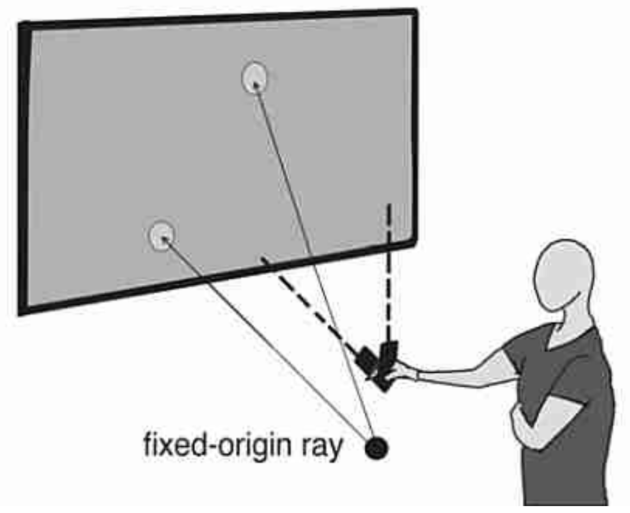
\includegraphics[height=6cm]{figures/related_work/pietroszek_2014_laser_pointer.png}%
  \caption[Laser pointer implementation by Pietroszek et al.]{
  The laser pointer interaction with a large display by \citeauthor{Pietroszek.2014}. Since the location of the smartphone is not known, the ray origin is set to a fixed position.
  \newline{}
  Source:~\cite[Figure 3]{Pietroszek.2014}}\label{fig:pietroszek-2014}
\end{figure}

To demonstrate the capabilities of the system, three-dimensional objects in the scene can be positioned and orientated. Finally, they conducted a study where they compare their system with a Wii controller. The results show no significant difference between those two input methods~\cite[125]{Pietroszek.2014}.

The ray casting system with the fixed-origin ray is also implemented in the laser pointer experiment presented later in this thesis.%, but to select objects in a \gls{VE} from \gls{VR}.


% Design and Implementation of an Immersive Virtual Reality System based on a Smartphone Platform
%\section{Design and Implementation of an Immersive VR System based on a Smartphone Platform}\label{section:design-implementation-vr-system-smartphone-platform}
\section{Steed et al.}\label{section:steed-2013}
The approach by \citeauthor{Steed.2013} also used a smartphone and a \gls{VR} headset as well as a visual representation of the phone. However, since they do not have positional tracking for the smartphone, the position is fixed relative to the position of the \gls{HMD}. There are two different possible positions, one in front of the users head (shown in Figure~\ref{fig:steed-2013-laser-pointer}) and the other one in front of the users belly (shown in Figure~\ref{fig:steed-2013-ui}). The position switches if a hand raise gesture with the phone in the hand is detected. Gestures and orientation of the smartphone are detected using the data of the \gls{IMU}.

\begin{figure}[H]
	\centering
	\begin{subfigure}[t]{0.45\textwidth}%
		\centering%
		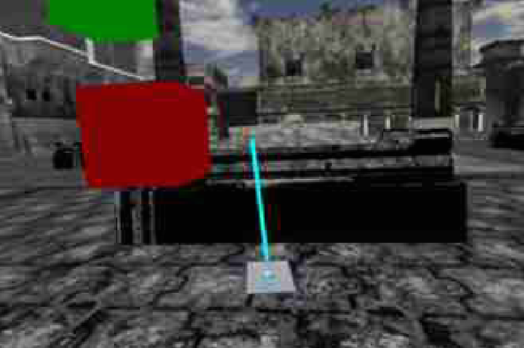
\includegraphics[height=4cm]{figures/related_work/steed_2013_laser_pointer.png}
		\caption{The virtual device in selection mode.}\label{fig:steed-2013-laser-pointer}% chktex 9 % chktex 10
	\end{subfigure}%
	\hspace{0.1\textwidth}%
	\begin{subfigure}[t]{0.45\textwidth}%
		\centering%
		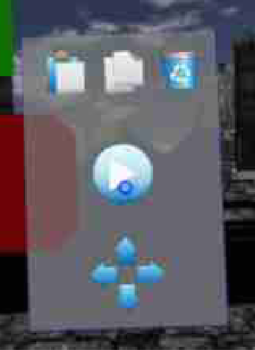
\includegraphics[height=4cm]{figures/related_work/steed_2013_ui.png}
		\caption{The virtual \gls{UI} and the cursor.}\label{fig:steed-2013-ui}
	\end{subfigure}%
  \caption[Virtual smartphone representation by Steed et al.]{The virtual smartphone representation by \citeauthor{Steed.2013}.
  \newline{}
  Source: Adapted from~\protect\cite[Figure 1]{Steed.2013}
  }\label{fig:steed-2013}
\end{figure}

On the virtual phone screen, a \gls{UI} is displayed as seen in Figure~\ref{fig:steed-2013-ui}. This \gls{UI} has control elements like buttons, which amongst others, can be used to toggle a selection mode. In the selection mode the phone casts a ray out of the top (similar to a laser pointer) as seen in Figure~\ref{fig:steed-2013-laser-pointer}. The ray direction can be changed by rotating the smartphone. As soon as a \gls{UI}-button is pressed, the objects intersecting with the ray are selected~\cite{Steed.2013}.

A similar laser pointer selection approach is implemented in one of the experiments in this thesis. The selection cursor and the fixed phone position also inspired the experiments presented in this thesis.


\section{Markussen et al.}\label{section:markussen-2013}
In {\citetitle{Markussen.2013}} \citeauthor{Markussen.2013} explore three different mid-air text input methods for large displays. Mid-air approaches track the users' hands and display a cursor on a external display. This method requires little to no visual attention of the users on their hands, because all the visual feedback is displayed on the large display. With common touch surfaces or displays, visual attention is required because the user has to aim for a virtual button or \gls{UI} element displayed on the touch device.
This approach also allows typing without restricting the users' movement around the display since the user does not have to touch any physical device~\cite[401]{Markussen.2013}.

The first approach, the \enquote{H4 Mid-Air} text entry method, allows to type using four buttons on a physical game controller. To type a character, a specific sequence of the four buttons has to be pressed in the correct order~\cite[406]{Markussen.2013}.

They also propose a reduced keyboard with nine buttons, where three to four characters are combined on one key (\enquote{MultiTap} approach). The user moves the cursor by moving his hand, which is tracked by a tracking system. When the cursor hovers over a key, the key is highlighted in orange -- the background of the key changes to red, when a key is activated. To type a character, the user taps a key multiple times in a certain time frame. The number of taps corresponds to the character's index on the key~\cite[407]{Markussen.2013}. % chktex 8

Their final method, \enquote{Projected QWERTY}, shown in Figure~\ref{fig:markussen-2013} uses a QWERTY\footnote{The name QWERTY describes the US layout for computer keyboards.} keyboard. It uses a similar cursor and highlighting as in the \enquote{MultiTap} approach, but only one tap is required to type a character. To determine the position of the cursor, the hand position is projected onto the display plane. This makes the cursor movement relative to hand movement independent of the distance from the hand to the display~\cite[408]{Markussen.2013}. 

\begin{figure}[H]%
	\centering%
	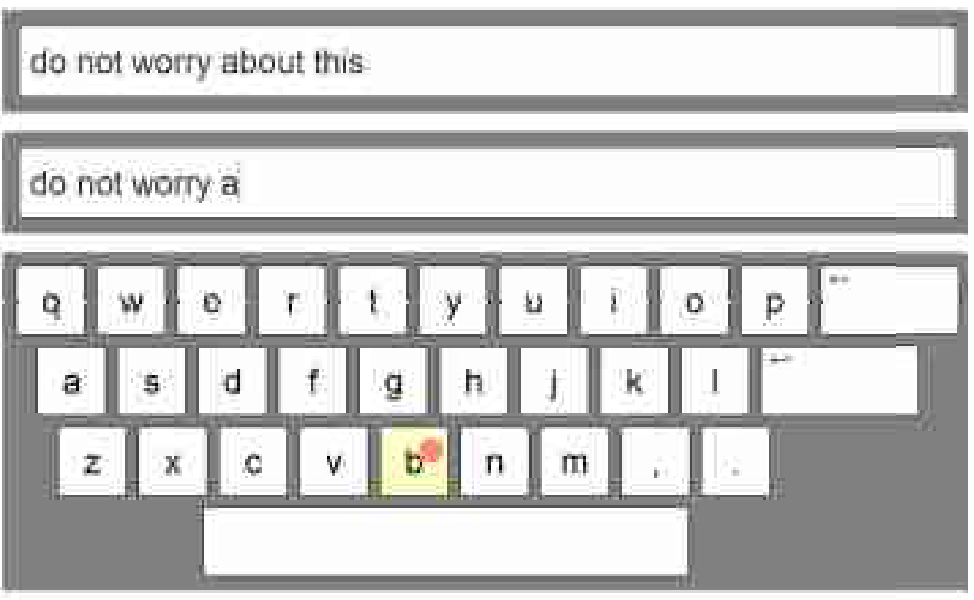
\includegraphics[height=6cm]{figures/related_work/markussen_2013_keyboard.png}%
  \caption[Virtual keyboard implementation by Markussen et al.]{
  The virtual keyboard of the user interface from the approach of \citeauthor{Markussen.2013}.
  \newline{}
  Source:~\cite[Figure 5]{Markussen.2013}}\label{fig:markussen-2013}
\end{figure}

A similar visibility-independent text entry method is used in this thesis to demonstrate a text input task for \gls{VR}.
